% Operations Manual Chapter Title
\infolevone{
\section{Introduction}
\label{sec:beam-intro}
}
% ESAD Section Title
\infoleveqnull{\section{Beamline}}

The control and measurement equipment along the Hall C beamline consists of
various elements necessary to transport beam with the required specifications
onto the reaction target and the dump and to simultaneously measure the
properties of the beam relevant to the successful implementation of the
physics program in Hall C.

\infolevone{
The resolution and accuracy requirements in Hall
C are such that special attention is paid to the following:
\begin{list}{\arabic{enumi}.~}{\usecounter{enumi}\setlength{\itemsep}{-0.15cm}}
  \item Determination of the incident beam energy;
  \item Control of the beam position, direction, emittance and stability;
  \item Determination of the beam current;
  \item Determination of the beam polarization.
\end{list}

Drawings of the Hall C line from the shield wall to the target are
shown in Figs.~\ref{fig:Cline1},~\ref{fig:Cline2},~ \ref{fig:Cline3}, and~\ref{fig:Cline4}.

\begin{figure}
\begin{center}
%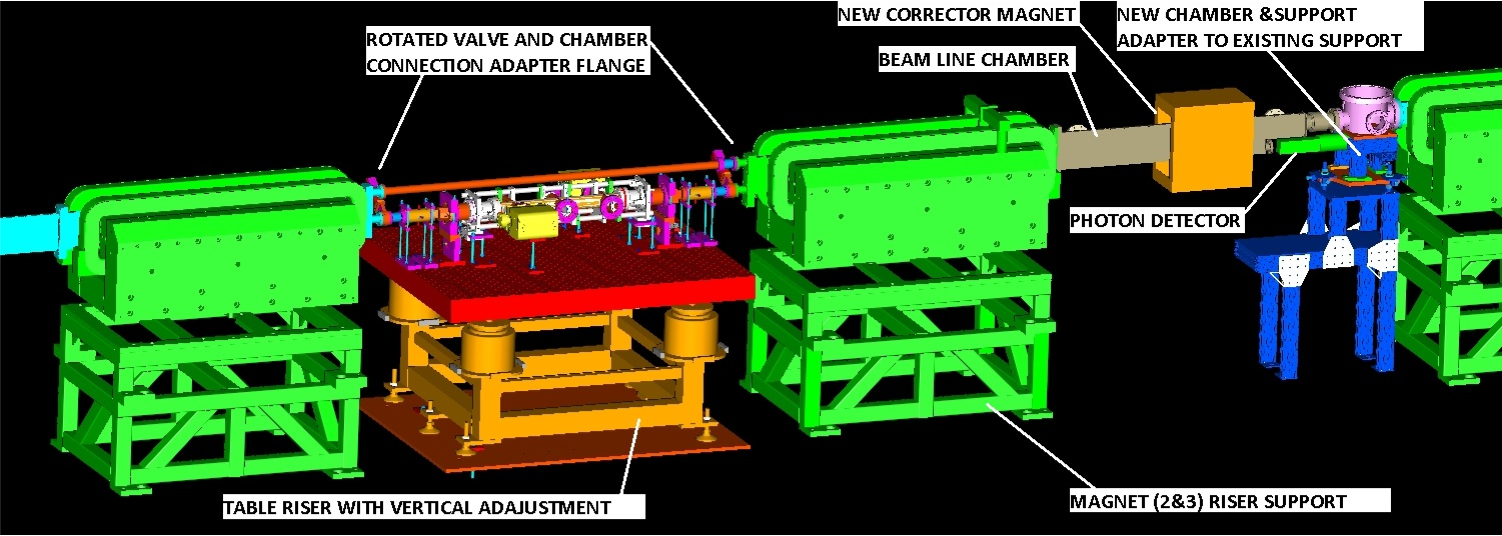
\includegraphics[angle=0,width=15cm]{compton_12gev.png}
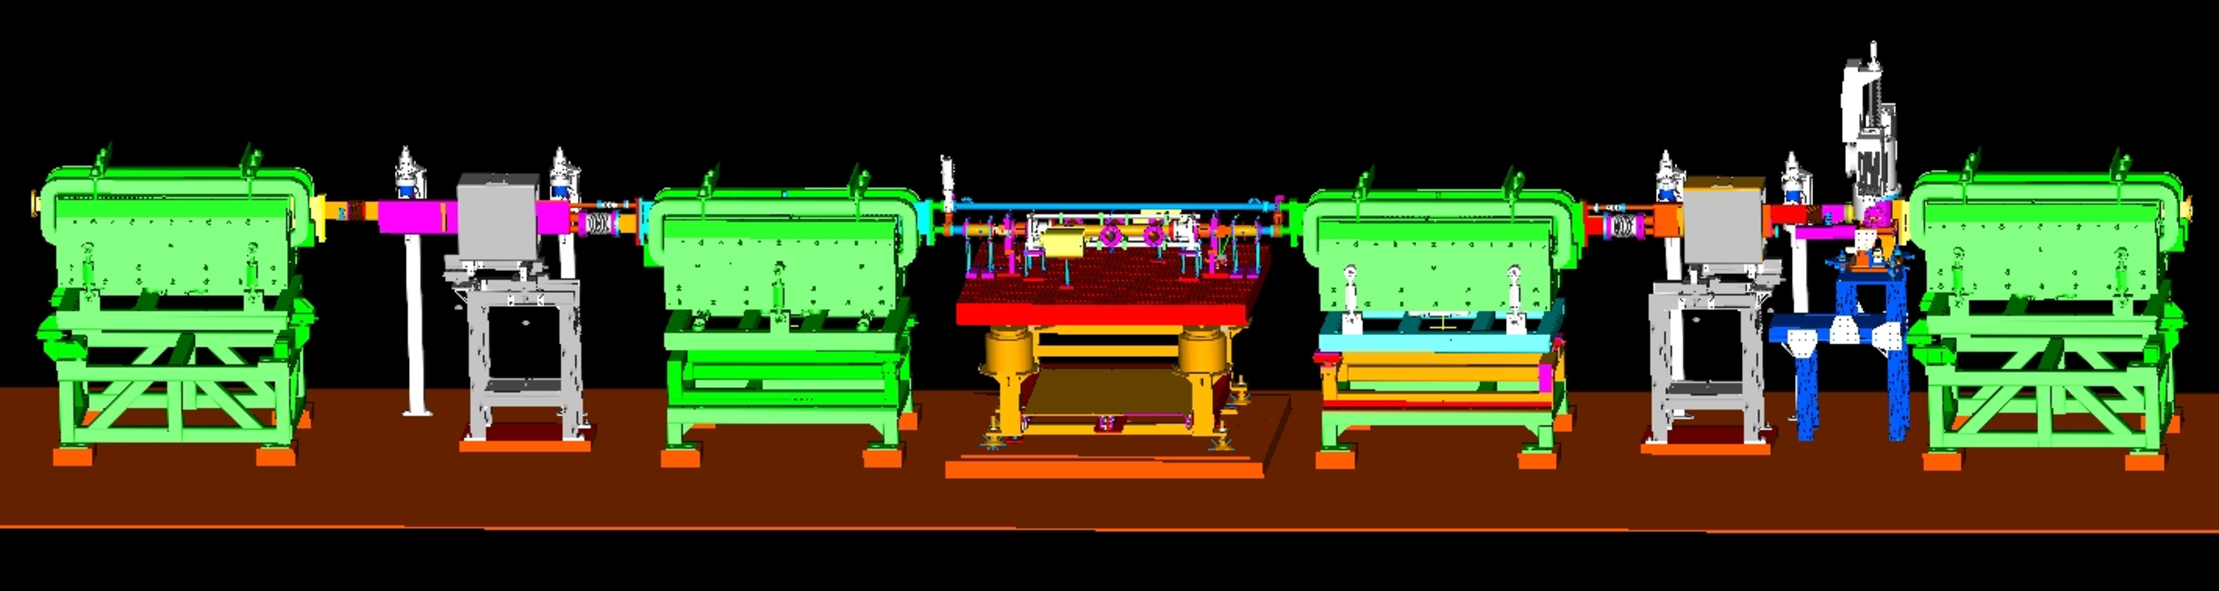
\includegraphics[angle=0,width=15cm]{compton_12gev_layout.pdf}
\caption[Beamline: Hall C Beamline Overview]{Compton Polarimeter, located
in the alcove.}
\label{fig:Cline1}
\end{center}
\end{figure}

\begin{figure}
\begin{center}
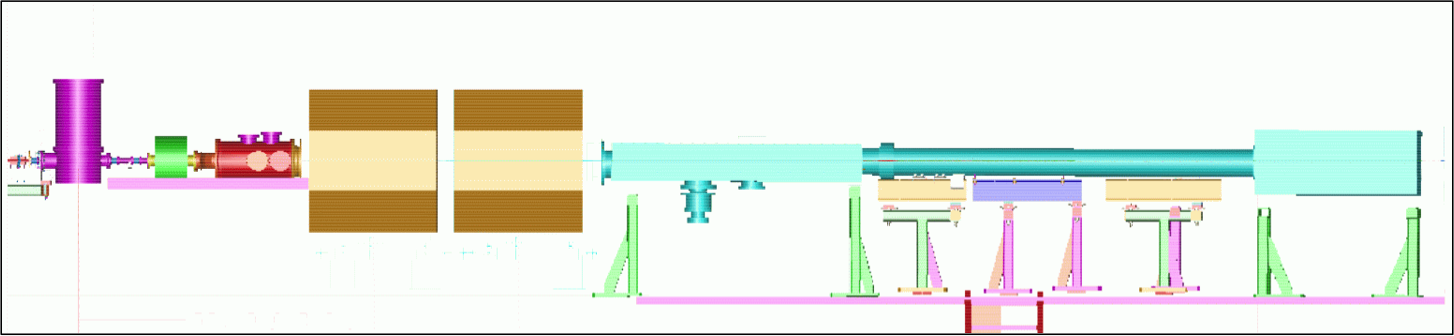
\includegraphics[angle=0,width=15cm]{moller_12gev.png}
\caption[Beamline: Hall C Beamline Overview]{Schematic of the Hall C
Moller Polarimeter, consisting of a superconducting magnet that polarizes
the Moller target, 3 quadrupole magnets that function as a spectrometer to
analyze Moller scattered electrons, and detectors.  The 3 quadrupoles also
serve as beam optics elements during normal operations.}
\label{fig:Cline2}
\end{center}
\end{figure}

\begin{figure}
\begin{center}
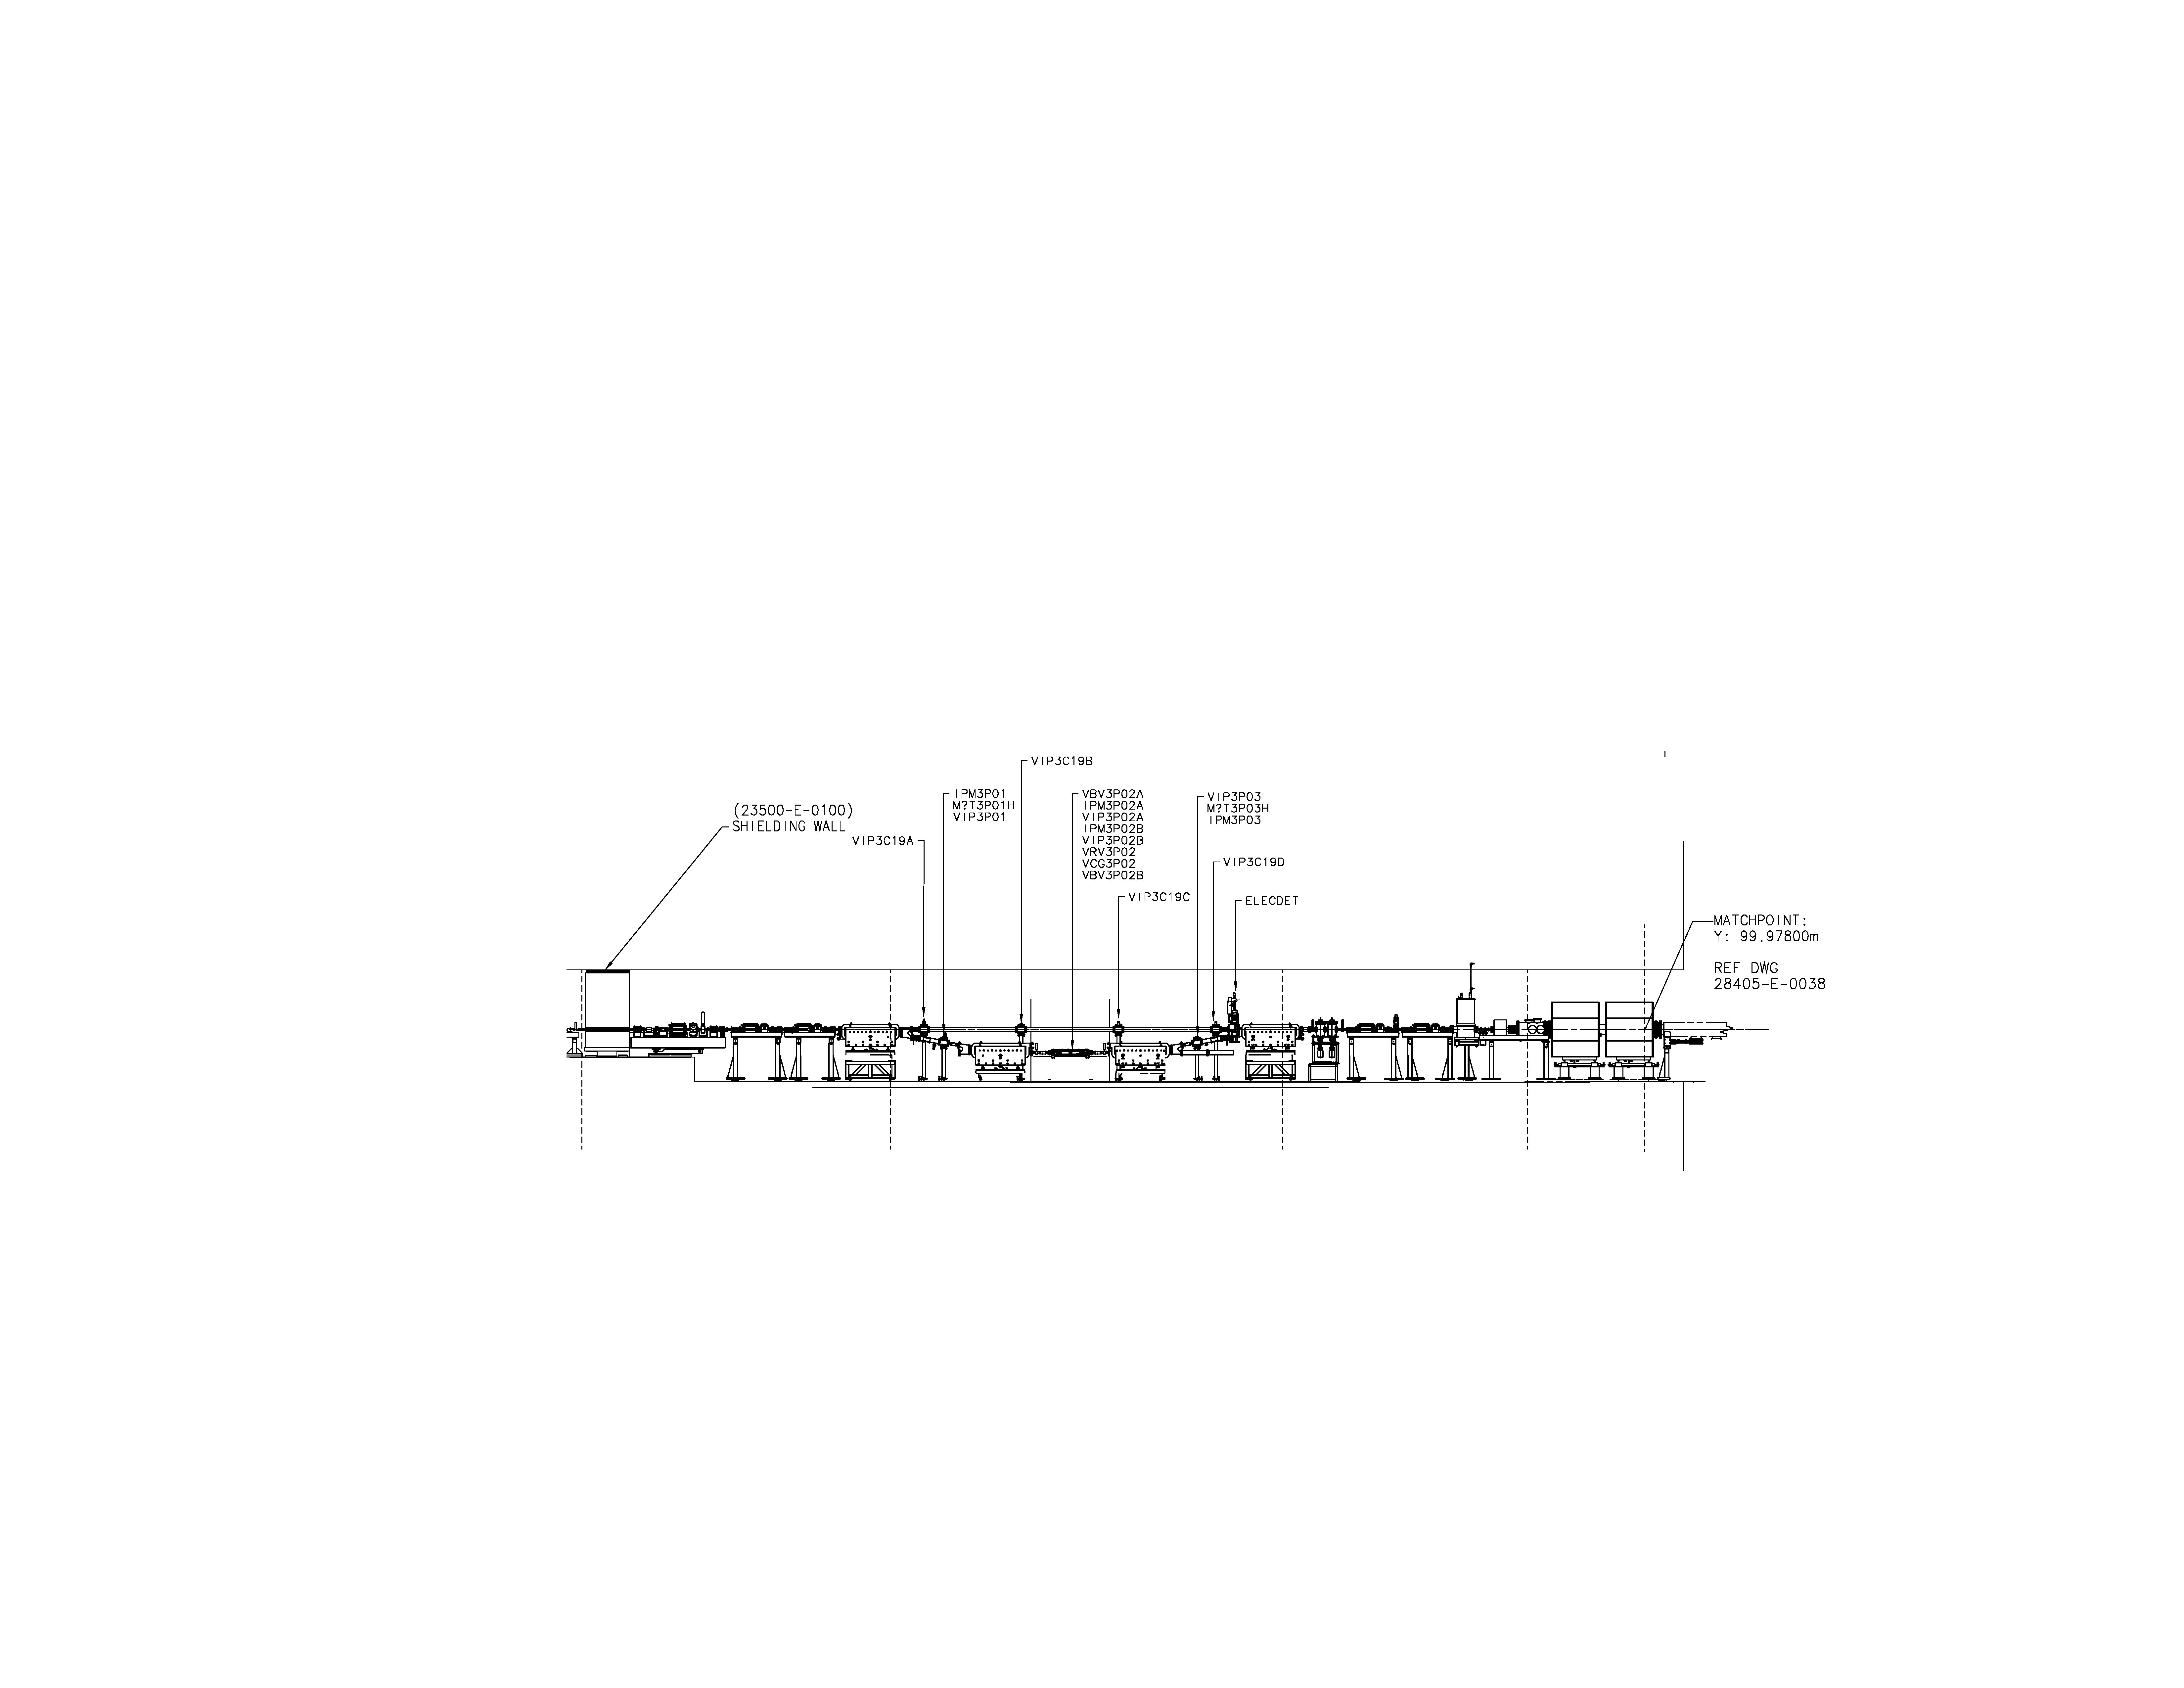
\includegraphics[angle=0,width=15cm]{hallc_beamline_arc_alcove.pdf}
\caption[Beamline: Hall C Beamline Overview]{Hall C beamline from green shield wall
to hall entrance.}
\label{fig:Cline3}
\end{center}
\end{figure}

\begin{figure}
\begin{center}
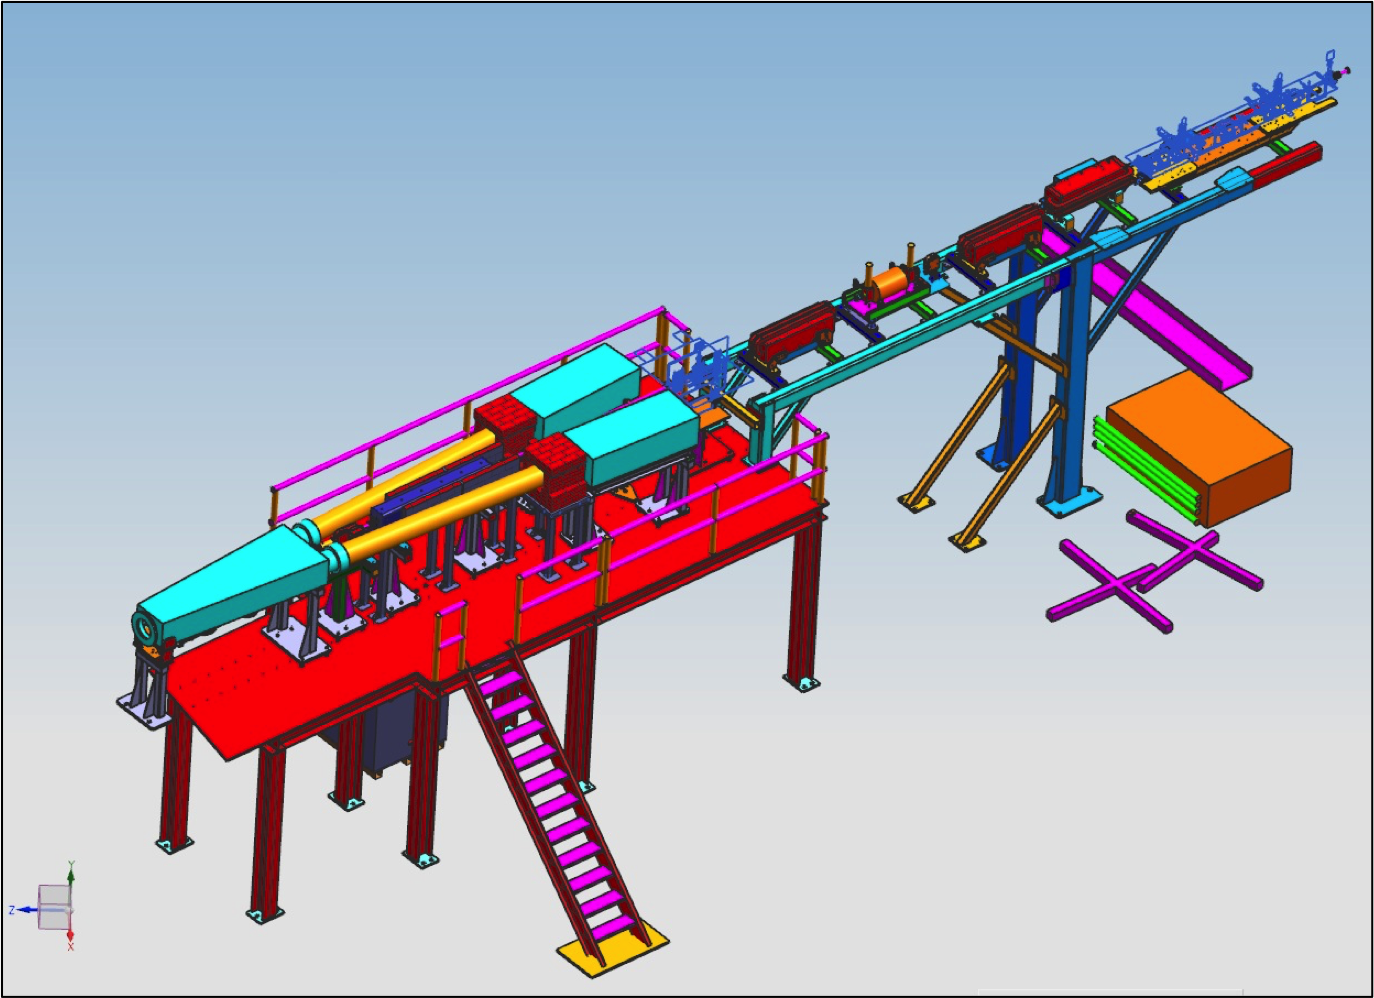
\includegraphics[angle=0,width=15cm]{ds_beamline.png}
\caption[Beamline: Hall C Beamline Overview]{View of the beamline from
entrance to the hall to the target scattering chamber.}
\label{fig:Cline4}
\end{center}
\end{figure}
}
\infolevfour{
The multiple elements in the beamline have a variety of ``owners''
and a variety of organizations with operational and fiscal
responsibilities.  These ownerships and responsibilities are
detailed in Fig.~\ref{fig:beamlineresponsibilities} and on the web \cite{blresp}.
\begin{figure}
  \begin{center}
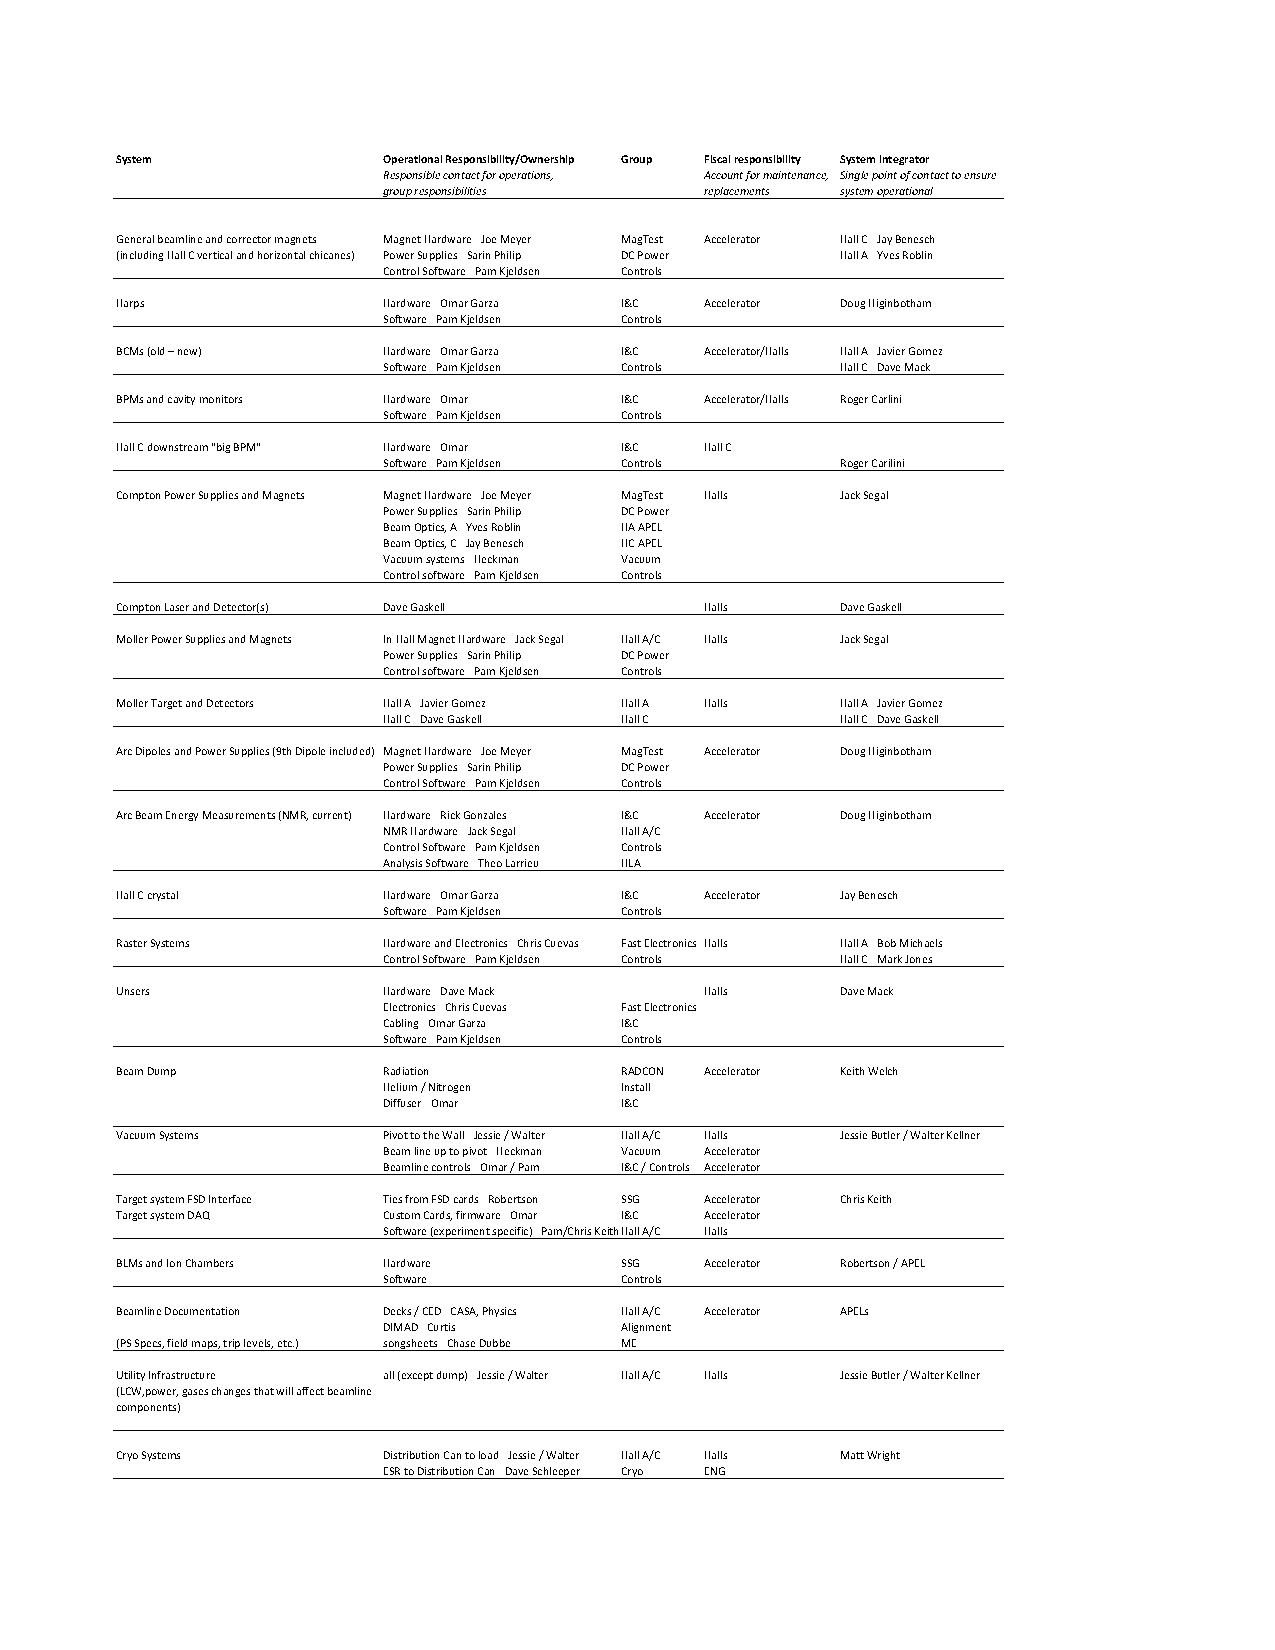
\includegraphics[width=1.1\textwidth,trim={0 1in 0 1in}]{Beamline_Responsibilities-3.pdf}
\caption{Beamline elements with operational and fiscal responsibilites.  The
most up to date version is maintained on the accelerator website \cite{blresp}.}
\label{fig:beamlineresponsibilities}
\end{center}
\end{figure}
}

\infolevtwo{
\subsection{The Beam Entrance Channel}

The beam entrance channel consists of 63.5 mm inner diameter stainless steel
tubing connected with conflat flanges. Through magnets the inner diameter of the
tubing is restricted to 25.4 mm.
Each section has a roughing port and is pumped with an ion pump.
The pressure is about 10$^{-6}$ Torr or better.


\subsection{The Beam Optics Channel}

These consist of dipoles, quadrupoles, sextupoles (generally not
used), and beam correctors with their standard girders and
stands. Starting from the beam switch yard, there are eight dipoles in
the arc section which (along with five other smaller beam deflectors)
bend the beam 37.5 degrees into the hall.
%Each dipole has a quadrupole
%and a pair of steering magnets (correctors) associated with it.
% Jay says: Each dipole does NOT have a quad and correctors associated
% with it.  MQ*3C 8,11,12,13,16 One quad each at start and end, three
% in the middle.  Gaps elsewhere. 
After
the shield wall at the entrance to the tunnel into the hall the beam
is essentially undeflected onto the target and into the dump. However
a small vertical displacement of the beam ($\approx$ 2 cm up) is
implemented to adjust the beam height to the optical axis of the Hall
C spectrometers.

The beamline optics elements are designed to deliver various optical
tunes of the beam on to the physics target as well as simultaneously
deliver various optical tunes at other locations along the
beamline. During normal operations, it is possible to deliver beam
with a focus at the physics target in the hall and at the interaction
point of the Compton polarimeter. It is not possible to simultaneously
achieve a focused beam at the M\o ller polarimeter target.

During normal operations, the beam is delivered with an achromatic
tune.  For measurement of the beam energy, a dispersive tune is
used. The nominal Hall C beam properties (achromatic tune) are listed
in Table \ref{beam_tab3}.

\begin{table}[hp]
\begin{center}
\begin{tabular}{|c|c|c|c|} \hline
{\bf Emittance}  & {\bf Energy Spread} & {\bf spot size}  & {\bf Halo}  \\
   (nm-rad)       &   $\sigma$ (\%)     & $\sigma$ ($\mu$m)&  (\%) \\ \hline
$\epsilon_x <$ 10 &  $<$ 0.05           & $\sigma_x<$ 400  &  $<$0.01 \\
$\epsilon_y <$ 5  &  $<$ 0.03           & $\sigma_y<$ 200  &        \\ \hline
\end{tabular}
\end{center}
\caption[Beamline: Hall C Beam nominal properties at target]{Hall C Beam nominal properties at target}
\label{beam_tab3}
\end{table}

\subsection{Beam Diagnostic Elements}

The key beam diagnostic elements consist of beam position monitors
(BPMs), beam current monitors (BCMs), and wire scanners (harps). Hall
C uses harps similar to those used throughout the CEBAF accelerator -
there are several harps placed in the Hall C beamline which provide
both absolute position and beam size information.  The harps at 3C07
and 3C17 are used as part of the beam energy measurement procedure.
The harp at 3C20 provides information relevant for the Compton and M\o
ller polarimeters. Finally the harps on the ``Hall C'' girder just
before the target (3CH07A and 3H07B) provide position information for
calibration of the BPMs and beam size information. All the harps in
the Hall C beamline are controlled by accelerator. When harp scans are
required for the experiment in the hall, shift workers should contact
MCC, request a scan of the relevant harp, and request that they post
the result in the electronic logbook.

To determine the position and the direction of the beam on the
experimental target point, three Beam Position Monitors (BPMs) are
located at distances 3.71 m (IPM3H07A), 2.25 m (IPM3H07B) and 1.23 m
(IPM3H07C) upstream of the target position.  The BPMs consist of a
4-wire antenna array of open ended thin wire striplines tuned to the
fundamental RF frequency of 1.497 GHz of the beam
~\cite{bi:bar90}. The standard difference-over-sum technique is then
used ~\cite{bi:HW} to determine the relative position of the beam to
within 100 microns for currents above 1 $\mu $A. The absolute position
of the BPMs can be calibrated with respect to the superharps which are
located adjacent to each of the BPMs (IHA3H07A at 3.46 m and IHA1H07B
at 1.55 m upstream of the target).

The BPMs are typically read out in two ways.
}

\infolevone{
1. The averaged position over 0.3 seconds is logged into the
EPICS~\cite{EPICSwww} database (1 Hz updating frequency) and injected
into the datastream every few seconds, unsynchronized but with an
reference timestamp. From these values we can consider that we know
the average position of the beam calculated in the EPICS coordinate
system which is left handed.

2. Event-by-event information from the BPMs are recorded in the CODA
datastream from each of the 8 BPM antennas (2x4) from which the
position of the beam can be reconstructed. However, these raw values
belong to a parallel electronics chain whose constants have to be
retrieved by calibrations to the EPICS or scanner data.

Figure~\ref{fig:bpm_readout} shows a schematic of how the BPMs are
read out for use in the Hall C data acquisition.

\begin{figure}
\begin{center}
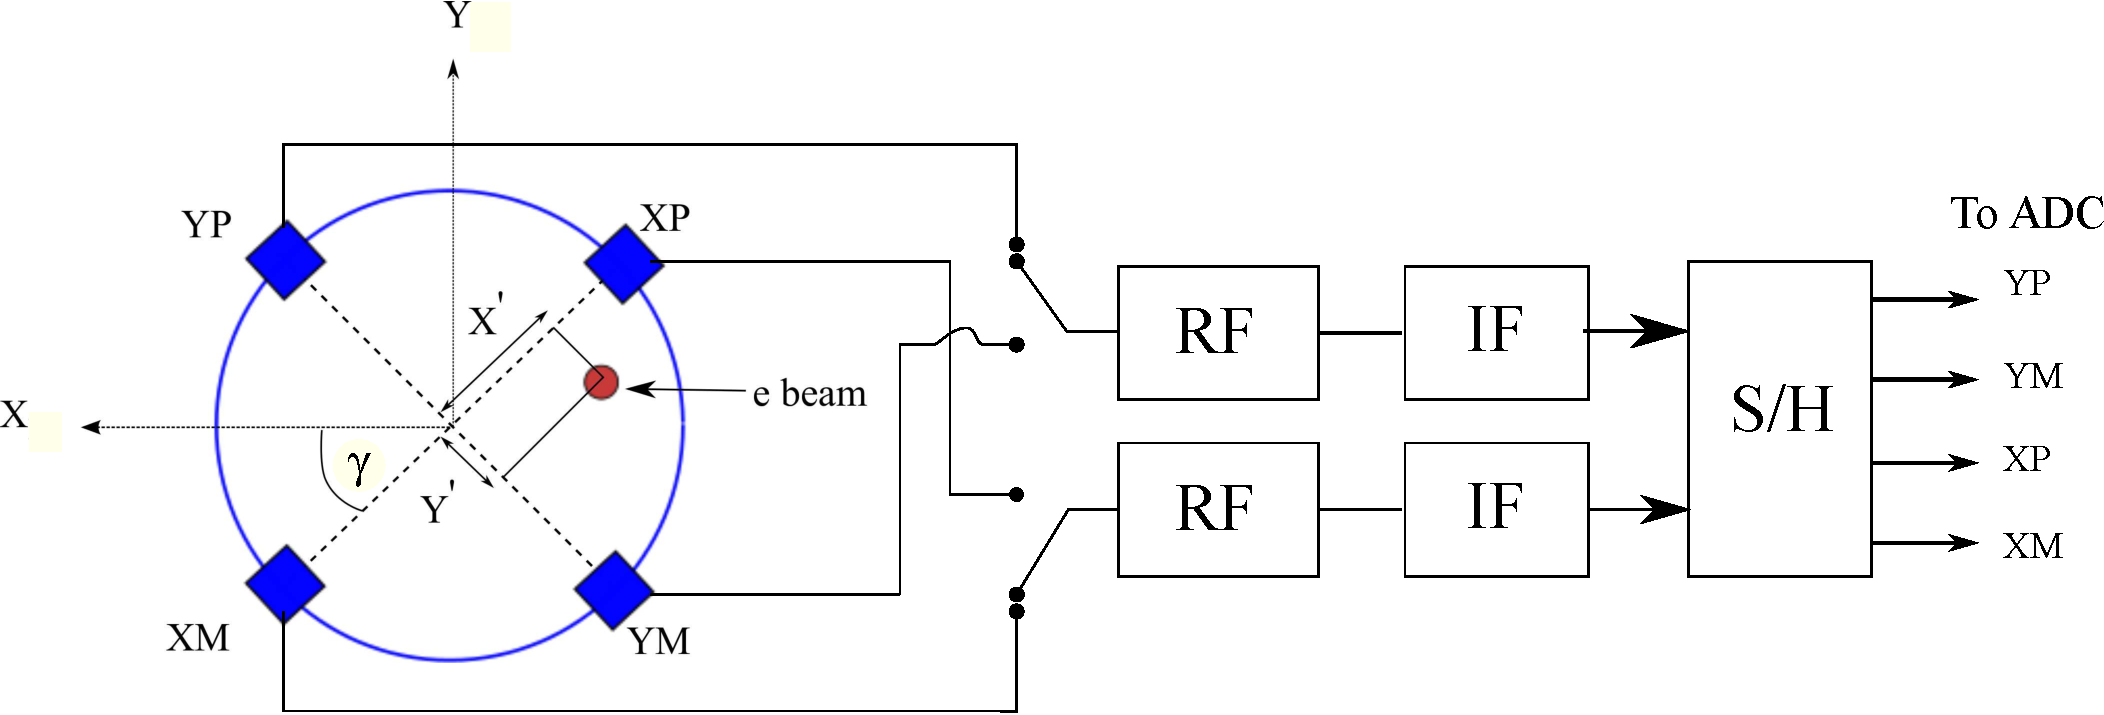
\includegraphics[angle=0,width=15cm]{bpm_electronics_chain.pdf}
\caption{Readout chain for the beam position monitors in Hall C.}
\label{fig:bpm_readout}
\end{center}
\end{figure}

In addition to measuring the beam trajectory before the target, it is also desirable
to measure the position and trajectory of the beam downstream because of the scattering
chamber because of potential steering effects from the fringe fields of the SHMS magnets
under certain operating conditions when the spectrometer is configured for small forward
laboratory angles.  To accomplish this two large diameter BPM’s (a.k.a. Big BPM’s) are
installed in the beam line as shown in Fig.~\ref{fig:ds_beamline}. These are mounted inside
dedicated 1.5m long removable sections of the 24” diameter downstream beam pipe. Their
mechanical structures, insulation materials and electrical connections to the outside are
constructed of extremely radiation hard materials (metals and ceramics). These devices are
designed to work with standard JLab BPM electronics.  Exact fit but hollow 24” beam pipe
replacement sections are available should removal or repair of these Big BPM’s be
desired/required. A cross-section sketch of a Big BPM is shown in Fig.~\ref{fig:big_bpm}.

\begin{figure}[htb]
\begin{center}
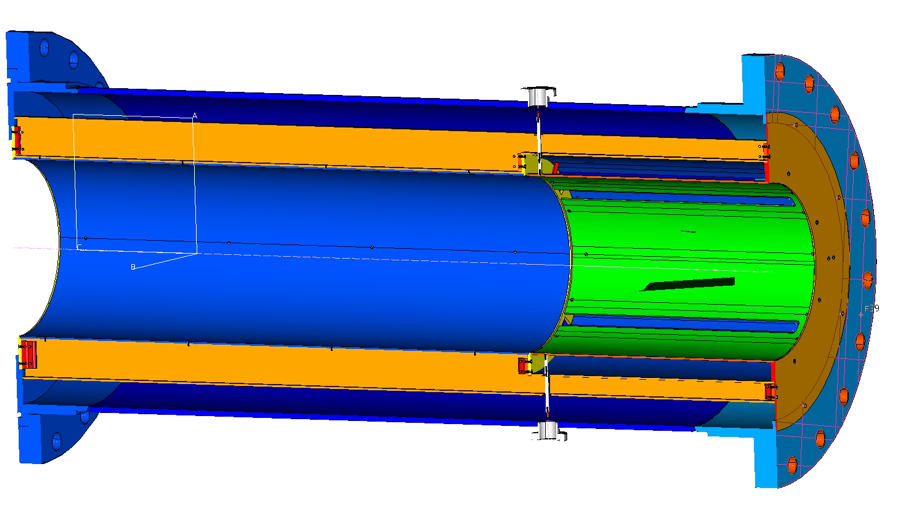
\includegraphics[angle=0,width=7cm]{big_bpm.png}
\caption{Cross-section of ``Big BPM'' to be installed in the beamline downstream
of the Hall C scattering chamber.}
\label{fig:big_bpm}
\end{center}
\end{figure}

\subsection{Beam Exit Channel}
% add figure for ds beamline?

After the target vacuum chamber, there is an exit beam pipe which
transfers the scattered beam onto the dump tunnel under vacuum. The
exit beam pipe will have more than one configuration due to the need
to accommodate the use of the smallest SHMS angle in some cases as
well as the pontential need to incorporate magnetic shielding to prevent the beam
from being deflected due to stray fields from the SHMS.

The downstream beam pipe has an overall length of about 90 feet from
the exit of the scattering chamber to the dump entrance. The portion
of the pipe closest to the dump entrance is made of several sections
of 24-inch diameter aluminum tube. As described earlier, some sections
of this 24-inch pipe can be replaced with sections to be used as beam
position monitors (BPMs). Closer to the target, the beam pipe steps
down to an 18-inch diameter tube. The combined length of the 18 and 24
inch diameter sections is about 44 feet.

Moving upstream the next section of pipe has a 6 inch diameter and is
about 23 feet long. The 16-feet long section between the scattering
chamber exit and the 6-inch diameter pipe is the region that undergo
the most potential configuration changes. Depending on the minimum
angles required for the SHMS and HMS, the beam pipe diameter can vary
from 1.5 to 4 inches. As noted earlier, special magnetic shielding
will be required when the SHMS is at small angles (typically less than
10 degrees), depending on the momentum.

An overview of the downstream Hall C beamline is shown in
Fig.~\ref{fig:ds_beamline}.

\begin{figure}
\begin{center}
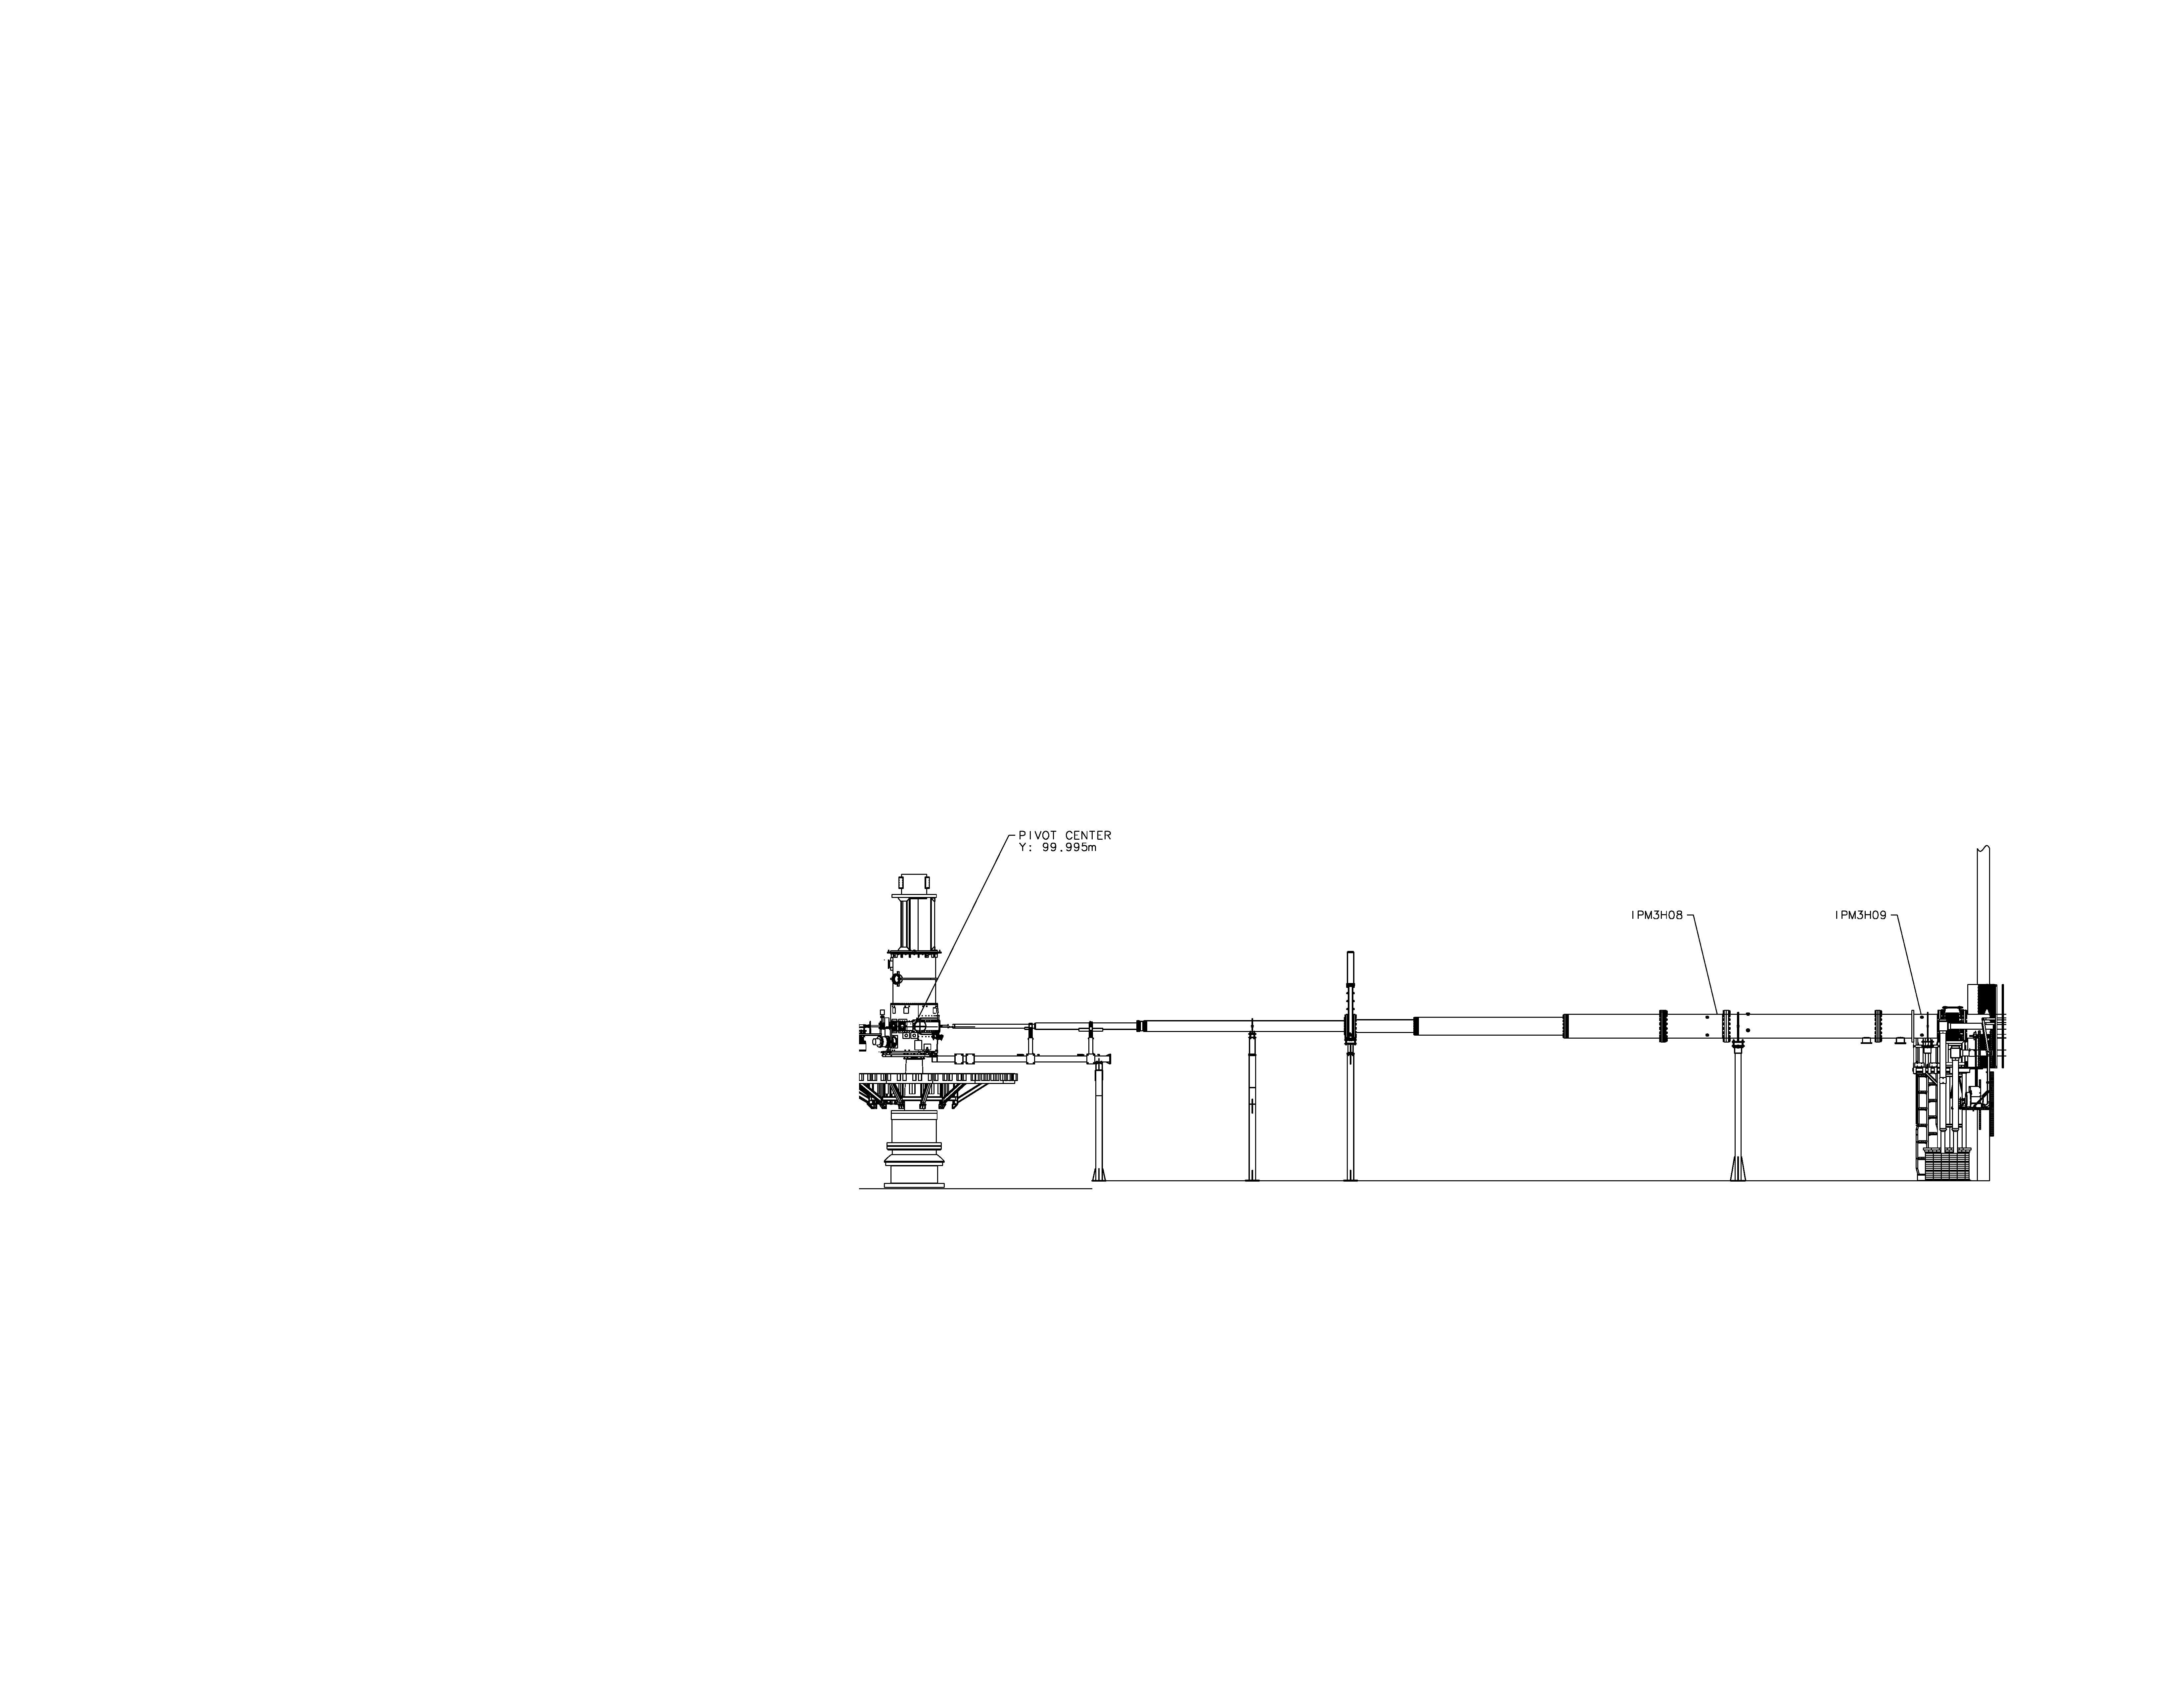
\includegraphics[angle=0,width=15cm]{hallc_ds_beamline_eng.pdf}
\caption{Schematic of the beam pipe that runs between the Hall C scattering chamber and the
beam dump entrance.}
\label{fig:ds_beamline}
\end{center}
\end{figure}

}

\infolevone{
\subsection{Machine/Beamline protection system}
\label{sec:beam-fsd}

The MPS~\cite{MPScebaf} system is composed of the Fast Shutdown System
(FSD), Beam Loss Monitor (BLM), and gun control system.

The FSD system is a network of permissive signals which terminate at
the electron gun and chopper 1. The permissive to the gun and chopper
1 may be inhibited by any device connected to an FSD mode. Devices
connected to the FSD system include vacuum valves, RF systems, Beam
loss systems, beam current monitors, beam dumps, and particular to
Hall C, the target motion mechanism and the raster.

The gun control system includes software program which monitors beam
operating conditions and the state of the FSD and BLM systems. the
program will warn the operators if a potential for beam damage
exists. Potential for damage exists when running high average current
beam, when FSD nodes are masked and when the beam power approaches the
operating envelope limits for a specific beam dump.  }

\begin{safetyen}{0}{0}
\infolevone{\subsection{Safety Information}}
%
% Information for the ESAD
%

The beamline in the Hall provides the interface between the CEBAF
accelerator and the experimental hall.  All work on the beamline must
be coordinated with both physics division and accelerator division; in
order to ensure safe and reliable transport of the electron beam to
the dump.

\infolevone{\subsubsection{Hazards}}
\infoleveqnull{\subsection{Hazards}}

Along the beamline various hazards can be found.  These include
radiation areas, vacuum windows, electrical hazards, magnetic fields
and conventional hazards.

\infolevone{\subsubsection{Mitigations}}
\infoleveqnull{\subsection{Mitigations}}

All magnets (dipoles, quadrupoles, sextupoles, beam correctors) and
beam diagnostic devices (BPMs, scanners, Beam Loss Monitor, viewers)
necessary for the transport of the beam are controlled by Machine
Control Center (MCC) through EPICS~\cite{EPICSwww}, except for special
elements which are addressed in the subsequent sections. The detailed
safety operational procedures for the Hall C beamline should be
essentially the same as the one for the CEBAF machine and beamline.\\

\noindent{}Personnel who need to work near or around the beamline should keep in mind the potential hazards:
\begin{itemize}
  \item Radiation ``Hot Spots'' - marked by ARM or RadCon
  personnel, \item Vacuum in the beam line tubes and other
  vessels, \item Thin windowed vacuum enclosures (e.g. the scattering
  chamber), \item Electric power hazards in vicinity of the
  magnets, \item Magnetic field hazards in vicinity of the magnets,
  and \item Conventional hazards (fall hazard, crane hazard etc.).
\end{itemize}

These hazards are noted by signs and the most hazardous areas along
the beamline are roped off to restrict access when operational.  In
particular, the scattering chamber, with it's large volume and thin
windows requires hearing protection once it has been evacuated.  Signs
are posted by RadCon for any hot spots along the beamline and RadCon
must be notified before work is done in a posted area.

Where appropriate (such as for the M\o ller polarimeter magnets),
magnet leads are covered with plastic guards for electrical safety.

\noindent{}Additional safety information is available in the following documents:
\begin{list}{--}{\setlength{\itemsep}{-0.15cm}}
  \item EH\&S Manual~\cite{EHScebaf};
  \item Personnel Safety System procedures~\cite{PSScontrolledenter,PSScontrolledexit,PSScontrolledproc};
  \item Accelerator Operations Directive~\cite{AODcebaf};
\end{list}

\infolevone{\subsubsection{Responsible Personnel}}
\infoleveqnull{\subsection{Responsible Personnel}}

Since the beamline requires both accelerator and physics personnel to
maintain and operate and it is very important that both groups stay in
contact that any work on the Hall C beamline is coordinated.

\begin{namestab}{tab:beam:personnel_beam}{Beam line: authorized personnel}{%
   Beamline physics division and accelerator division points-of-contact.}
  \namestabheader{Hall C Physicists}
  \DaveGaskell{\em 1st Contact}
  \MarkJones{\em 2nd Contact}
  \namestabheader{Liaisons from Accelerator Division}
  \HariAreti{..to Physics}
  \JayBenesch{..to Hall-C}
\end{namestab}
\end{safetyen}
